\documentclass{article}

\usepackage{multicol}
\usepackage{titlesec}
\usepackage{graphicx}
\usepackage{wrapfig}

\graphicspath{{./images/}}

\title{Physics Unit}
\author{Anna Denisova}
\date{2023}

\begin{document}

\maketitle
\tableofcontents

\newpage

%-------------------------------------------------------------------------------------------------------------

\section{Static Electricity (pg. 465)}

    \subsection*{Atomic Structure and Electric Charge}

    \begin{itemize}
        \item All matter is made up of \textbf{atoms} 
        \item Atoms contain \textbf{protons} (+), \textbf{neutrons} (0), \textbf{electrons} (-)
        \item Atoms have no charge, while ions have positive charges (\textbf{cation}) or negative charges (\textbf{anion})
        \item Only electrons can transfer
    \end{itemize}

    \subsection*{Positive, Negative, and Neutral Objects}

    We use + and - signs to represent an equally large group of protons and neutrons respectively. \textit{The overall charge of an object can be determined by comparing the number of + and - signs drawn on the object.}\\
    
    \noindent
    The \textbf{transfer of electrons} between objects can both charge neutral objects and neutralize charged objects. Most of the objects we interact with on a daily basis are neutral.

    \subsection*{Static Electricity}
    \textbf{Static electricity} is an imbalance of electric charges on the surface of a material or between materials. This produces a \textbf{static chrage}, as the charges stay at rest on the surface of the object.\\

    \subsection*{The Law of Electric Charges}

    \begin{itemize}
        \item A charged object exerts an electric force, which can be either an attractive force or a repulsive force
        \item Objects with \textbf{like charges repel each other}
        \item Objects with \textbf{opposite charges attract each other}
        \item The strength of the electric force increases with increasing electrical charges and decreases with increasing distance
    \end{itemize}

    \subsection*{Attraction of Neutral Objects to Charged Objects}
    
    \begin{itemize}
        \item A neutral object has no charge (if two netural objects are brought near each other, nothing happens)
        \item According to the \textbf{Law of Electric Charges}, when a charged object is brought near a neutral object, it induces the electrons \textit{to shift in position}, which is called \textbf{induced charge separation}
        \item No electrons are gained or lost in this process; the electrons return to their original positions once the charged object is moved away from the neutral object
    \end{itemize} 

    \subsection*{Detecting Static Electric Charges}

    One way is to use an \textbf{electroscope} to detect the presence of electric charges.

    \subsubsection*{Pith Ball Electroscope}
        Consists of a ball of bith (plant material) suspended from a strand by a thread. To test for the presence of an electrical charnge on an object, it is brought near the neutral bith ball. If the object is charged, the pith ball will be attracted to it.\\
        \begin{center}
            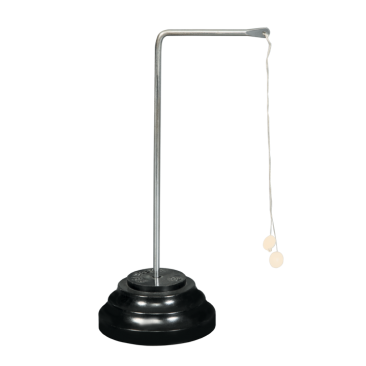
\includegraphics[scale = 0.3]{pithball electroscope}
        \end{center}

    \subsubsection*{Metal Leaf Electroscope}

        More sensitive to electric charge than a pith ball electroscope.
        It consists of a vertical rod with two thin pieces of metal foil called "the leaves". The object is brought near the metal terminal attached to the top of the rod to test for a charge. If the object is charged, electrons are transferred to (or from) the leaves of the electroscope, which charges the leaves, causing them to repel each other.
        \begin{center}
            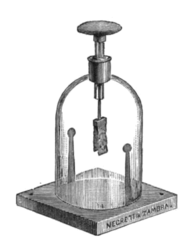
\includegraphics[scale = 0.3]{electroscope}
        \end{center}
        \begin{center}
            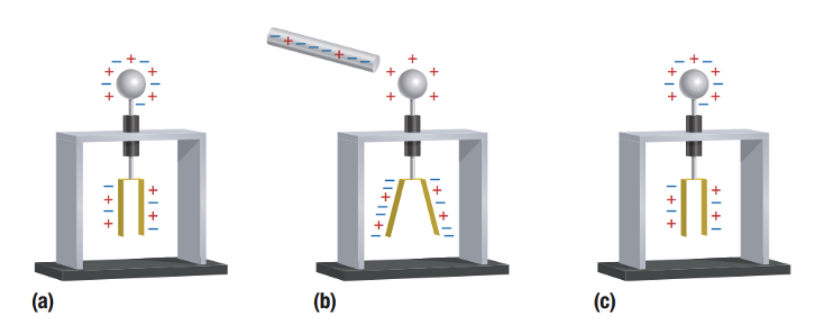
\includegraphics[scale = 0.6]{metal leaf electroscope}
        \end{center}
        

    \subsection*{Using Static Charges}
    
    \begin{itemize}
        \item Electrostatic paintsprayers
    \end{itemize}

%-------------------------------------------------------------------------------------------------------------

\newpage

\section{Charging by Contact (pg. 273, pg. 472)}

    \subsection*{Charging Objects by Friction}

    \textbf{Occurs when two different neutral materials are rubbed together or come in contact.}\\\\
    One object is more likely to become negatively charged while the other is more likely to become positively charged (some atoms are more strongly attracted to electrons than others).\\\\
    Objects become charged more easily in the winter than in the summer since the air is more humid in the summer (water molecules in the water vapor collide with nearby objects, tranferring the electrons from the charged object to the water molecules, thus causing the object to lose its charge). \\

    \subsection*{The Electrostatic Series}

    \noindent
    \begin{wrapfigure}{r}{0.25\textwidth} %this figure will be at the right
        \centering
        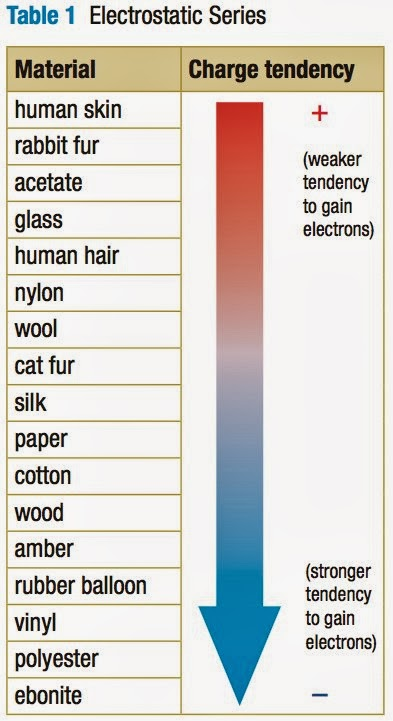
\includegraphics[scale = 0.13]{electrostatic series}
    \end{wrapfigure}

    \begin{flushleft}
        \textit{This is a list of materials in order of increasing tendency to gain electrons. The lower the material is in the list, the greater the tendency to gain electrons.} This is used to predict the charge that will be gained by two objects or materials that are rubbed together; the one higher on the list will lose electrons and become positively charged while the one lower on the list will gain electrons and become negatively charged. \\
    \end{flushleft}

    \subsection*{Charging Objects by Conduction}
    \textbf{Occurs when two objects with different amounts of electric charge come in contact and electrons move from one object to the other.}\\
    The objects are either both charged or one is charged and one is neutral, as long as they have different charges.\\\\
    Electrons move from the object with a larger negative charge to the object with a smaller negative charge so that both objects will have an equal charge; essentially, the charges are averaged.\\

    \subsubsection*{Example}
    If a piece of metal has a charge of +3 and other peice of metal has a charge of + 1, they will both end up with a charge of + 2 after coming in contact.\\\\
    The charge is NOT neutralized, rather, both objects have the same type and amount of charge. \\
   
    \subsubsection*{Grounding}
    A process which involves removing an object's excess charge by transferring \textbf{electrons between the object and a large neutral object} such as Earth (the ground). \\\\
    Any object that serves as a seemingly infinite reserrvoir of electrons can be used as a "ground" for electric charges; Earth effectively neutralizes any excess charge since it spreads out over a huge area.\\\\
    When grounded, electrons travel from the ground to the object if it is positively charrged, and vice versa if it is negatively charged.\\

    \subsubsection*{Putting Charged Objects to Work}
    \begin{itemize}
        \item \textbf{Electrostatic dusters} depend on charging by friction to operate. Charge builds up as the duster is swept across an object, causing the dust to become attracted to the duster and move off of the dusty surface to the duster.
        \item Ostrich feathers have a natural tendency to become charged when rubbed
        \item \textbf{Electrostatic precipitators} are used in large power plants, manufacturing plants, and incinerators to remove particles from the air. The particles in the smoke become negatively charged by conduction as the smoke passes through the negatively charged plates. The particles then stick to positively charged plates as they pass through them and fall onto the collection plate, allowing them to be removed.
        \begin{center}
            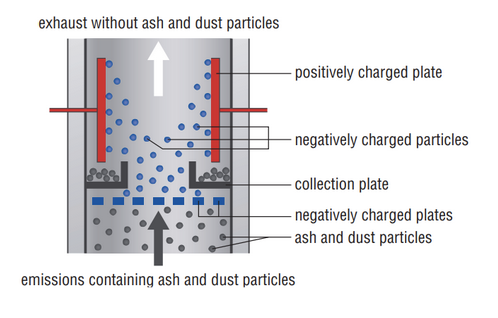
\includegraphics[scale = 0.7]{electrostatic precipitator}
        \end{center}

    \end{itemize}




%-------------------------------------------------------------------------------------------------------------

\section{Conductors and Insulators (pg. 480)}

    \textbf{Conductors} are materials that allow the movement of electrons.\\
    \textbf{Insulators} are materials that prevent the movement of electrons.\\
    
    \subsection*{Conductors}
    \begin{itemize}
        \item \textbf{Good conductors} allow electrons to move through them with easy
        \item \textbf{Fair conductors} allow electrons to move through them with a small amount of difficulty
        
        %insert img here

        \item Graphite and silicon are \textbf{semiconductors} because they allow electrons to move through them, although not as easily as in a good conductor
        \item It is not possible to place a charge on a conductor if it is in your hand since it would immediately pass through the conductor into your hand
        \item Water is generarlly conductive and should therefore not be near electrical appliances when you are handling them, as you are at risk of injury from the movement of large amount of electric charge through your body
        \item Pure water, which has no ions, is not conductive
    \end{itemize}

    \subsection*{Insulators}

%-------------------------------------------------------------------------------------------------------------

\section{Charging by Induction (pg. 286)}

    \subsection*{Charging Objects Temporarily by Induction}
        
%-------------------------------------------------------------------------------------------------------------

\section{Electric Circuits (pg. 509)}

%-------------------------------------------------------------------------------------------------------------

\section{Forms of Current Electricity (pg. 515, 551)}

%-------------------------------------------------------------------------------------------------------------

\section{Electric Current and Potential Difference (pg. 556)}

%-------------------------------------------------------------------------------------------------------------

\section{Ohm's Law (pg. 568)}

%-------------------------------------------------------------------------------------------------------------

\section{Current and Voltage in Series and Parallel Circuits (pg. 571)}

%-------------------------------------------------------------------------------------------------------------

\section{Electrical Power and Efficiency (pg. 530)}

%-------------------------------------------------------------------------------------------------------------

\section{Power and Efficiency}

%-------------------------------------------------------------------------------------------------------------

\section{Generating Current Electricity (pg. 518)}

%-------------------------------------------------------------------------------------------------------------

\end{document}